\chapter{Introduzione}

In questo capitolo verranno descritte rapidamente le regole del gioco \cite{mafiaWikipedia} sul quale si basa il sistema e le caratteristiche che quest'ultimo avrà.

\section{Regole del gioco}
Lo svolgimento del gioco si basa sull'alternarsi di fasi diurne e notturne nelle quali i diversi personaggi potranno intraprendere azioni specifiche. E' presente un narratore con il compito di supervisionare l'alternarsi delle fasi di gioco, tenere traccia delle decisioni dei giocatori e delle loro azioni.\\[\baselineskip]\indent
Nella versione originale e più semplice del gioco i ruoli sono quelli di \emph{villico} e \emph{lupo}, per cui si andranno a creare due squadre con obiettivi contrapposti, identificare i lupi ed uccidere i villici. Ad ogni turno di notte il narratore dovrà chiedere ai lupi chi vogliono uccidere all'insaputa dei villici, successivamente poi chiederà ai vari personaggi "extra" di compiere azioni specifiche associate ai vari ruoli, mentre durante il turno di giorno tutti i giocatori dovranno decidere chi accusare di essere un lupo, consapevoli però che i lupi cercheranno di influenzare a loro favore la decisione. \\[\baselineskip]\indent
La partita termina nel momento in cui i giocatori di una delle due squadre hanno la meglio sugli altri, avendo identificato ed accusato correttamente tutti i lupi per la squadra dei villici o rimanendo in superiorità numerica per la squadra dei lupi. A questo punto sarà sufficiente distribuire nuovamente i ruoli per iniziare una nuova partita.

\section{Descrizione del sistema}

Il sistema ricoprirà il ruolo di narratore nella partita, permettendo così lo svolgimento del gioco anche nel caso in cui i giocatori non si trovino fisicamente nello stesso luogo.\\
A monte di questa funzionalità il sistema dovrà permettere l'autenticazione dei giocatori attraverso credenziali e tenere traccia delle loro informazioni. I giocatori potranno poi formare un \emph{party} di gioco privato all'interno del quale avviare le singole partite.

Una volta che il numero minimo di giocatori minimo di giocatori viene raggiunto sarà possibile decidere le configurazioni di gioco, impostando il numero di lupi e l'eventuale presenza di ruoli extra, scegliendo tra quelli preimpostati.
Avviando la partita il sistema si occuperà di assegnare in maniera casuale i ruoli ai giocatori dando poi il via al primo turno, ovvero alla prima \emph{notte}.\\[\baselineskip]\indent
Lo svolgimento del gioco procede poi in maniera automatica, ciclando i turni previsti e richiedendo ai giocatori di effettuare delle scelte qualora sia il loro turno. 

Qualora si verifichino le condizioni necessarie per considerare una delle due fazioni vincente allora il sistema porrà fine alla partita indicando i vincitori ed i perdenti, dando poi la possibilità di salvare la partita appena effettuata al fine di raccogliere statistiche per tutti i partecipanti.
Il \emph{party} potrà quindi decidere di ridistribuire i ruoli e giocare nuovamente oppure ritornare alla pagina iniziale.

\begin{figure}[H]
\centering
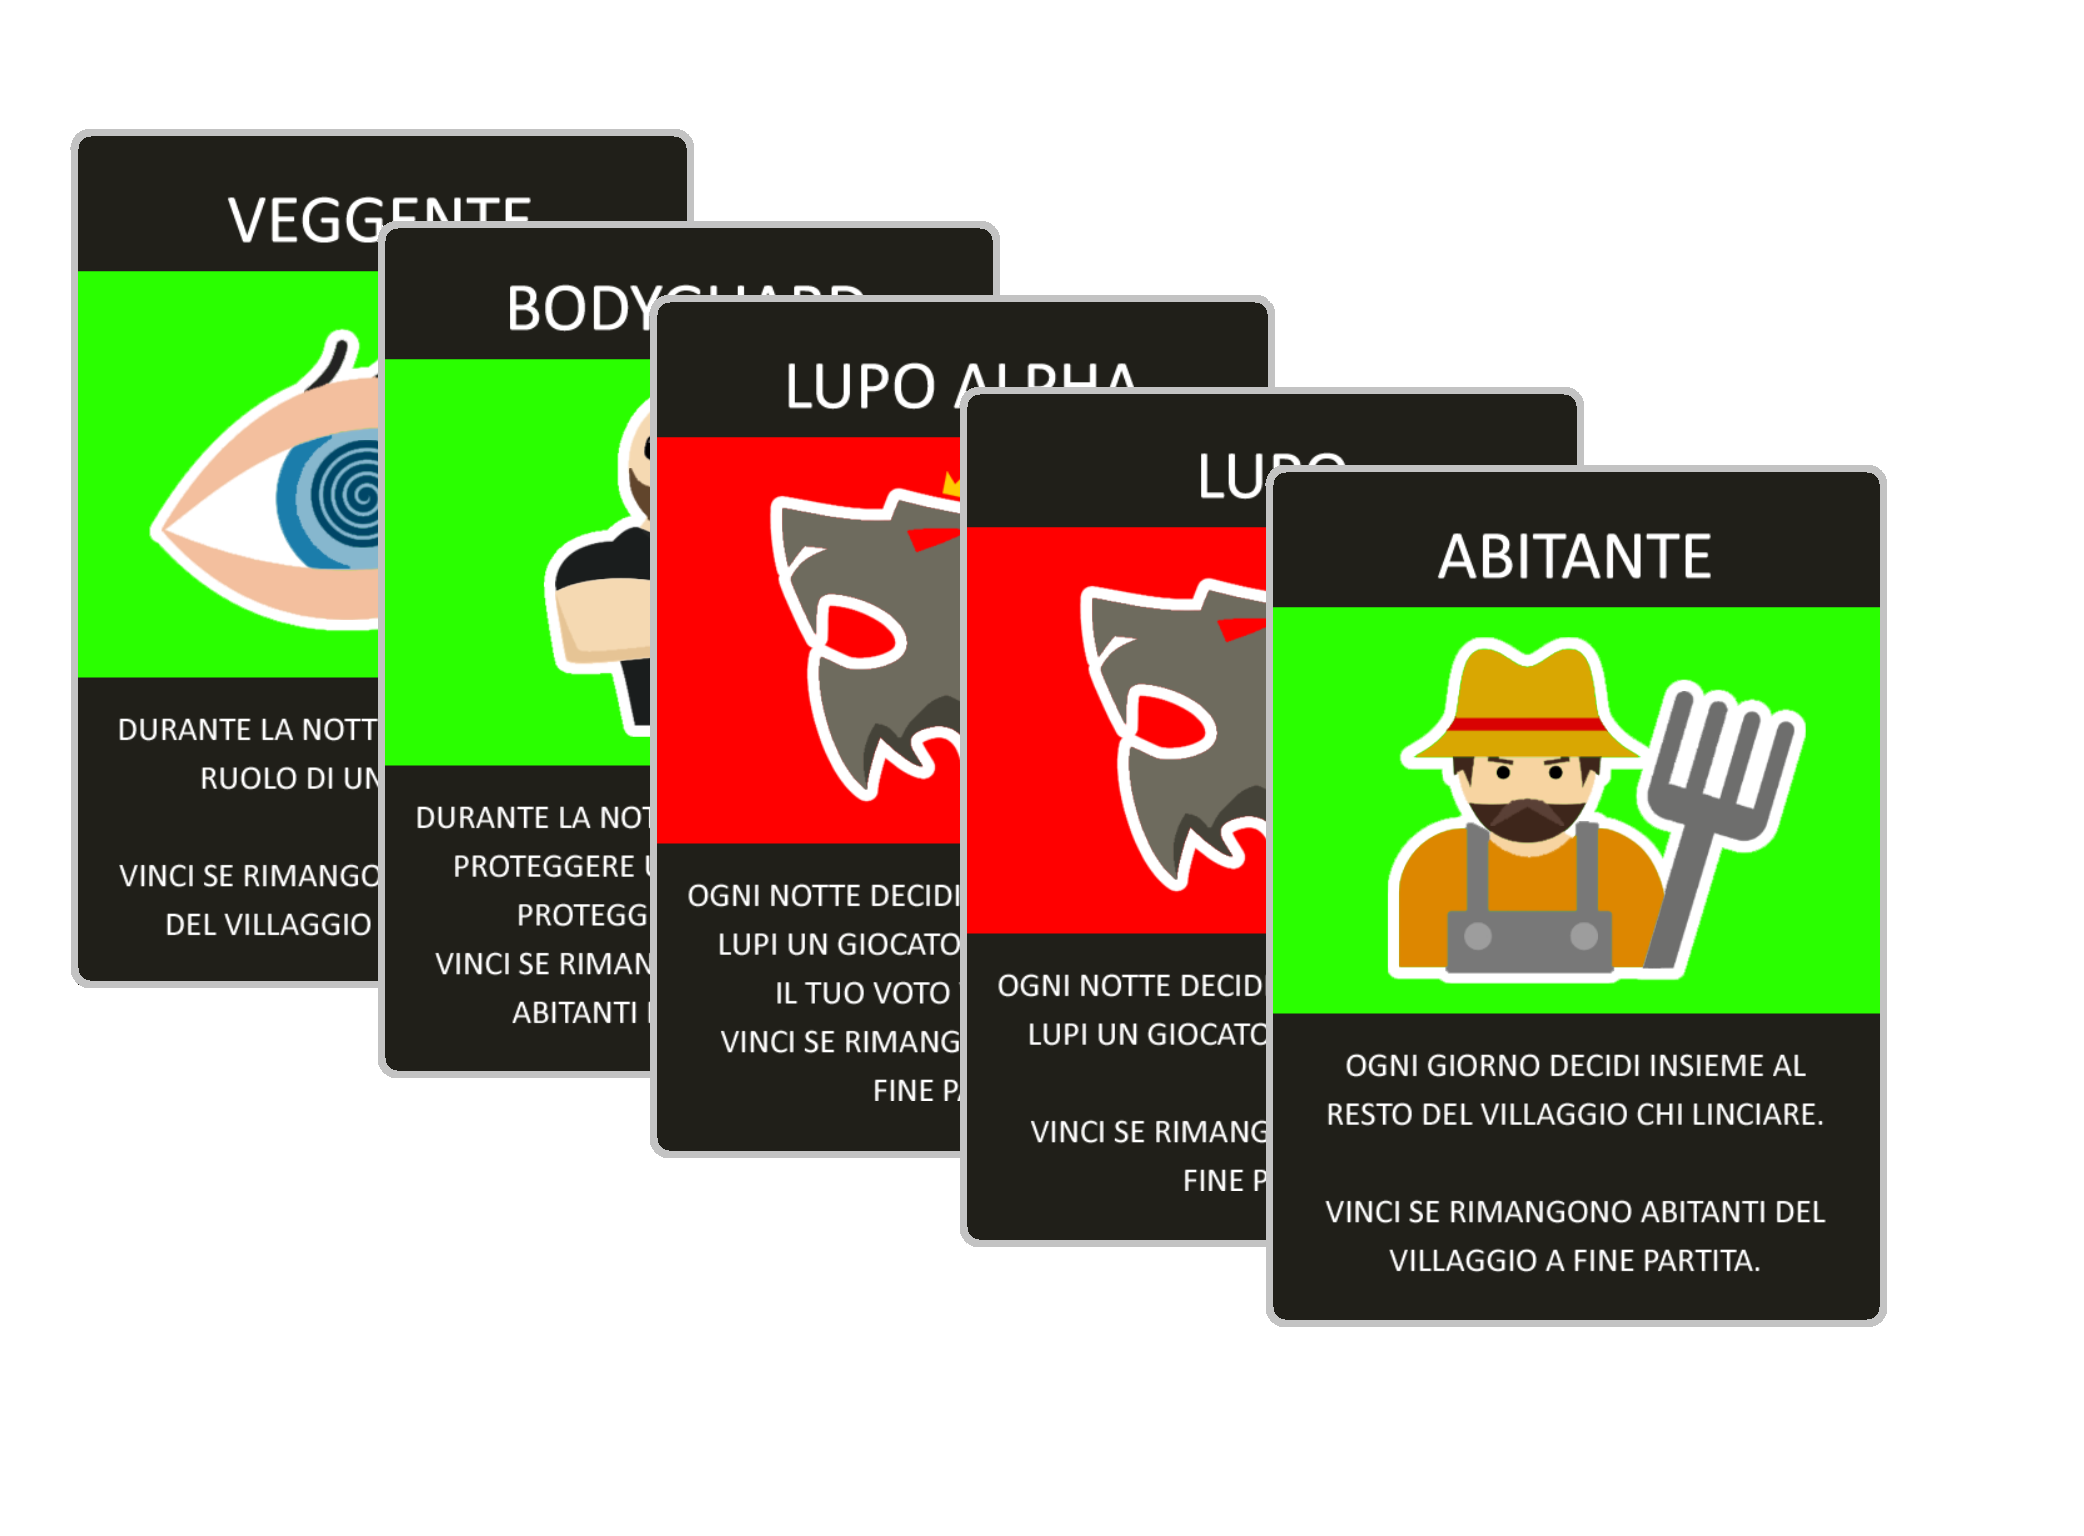
\includegraphics[width=\textwidth]{img/cards.png}
\caption{Ruoli implementati in Lupus}
\label{fig:cards}
\end{figure}